
%\typeout{How Anthropomorphic Design Shapes Information Use in Conversational Agents: A Meta-Analysis of 79 Empirical Studies}
\typeout{The Effect of Anthropomorphic Design of Conversational Agents on User Outcomes: A Meta-Analysis of 79 Empirical Studies}

% These are the instructions for authors for IJCAI-24.

\documentclass[preprint,review,12pt,authoryear,nonatbib]{elsarticle}
% Use the postscript times font!
\usepackage{times}
\usepackage{soul}
\usepackage[utf8]{inputenc}
\usepackage[small]{caption}
\usepackage{subcaption}
\usepackage{graphicx}
\usepackage{amsmath}
\usepackage{amsthm}
\usepackage{booktabs}
\usepackage[switch]{lineno}
\usepackage{multirow}
\usepackage[ruled,vlined]{algorithm2e}
\usepackage[breakable]{tcolorbox}
\usepackage{listings}
\usepackage{csquotes}
\usepackage[
    backend=biber,
    style=apa,
    sorting=nyt,
    sortcites=true
]{biblatex}

\DeclareLanguageMapping{english}{english-apa}
\addbibresource{references.bib}

\usepackage{url}
\usepackage{longtable}
\usepackage{setspace}
\usepackage{float}
\usepackage{hyperref} 
\usepackage{tabularx}
\usepackage{xcolor}
\usepackage{pgfplots}
\pgfplotsset{compat=1.18}
\usepackage{siunitx}
\usepackage[table]{xcolor}

\definecolor{changeblue}{RGB}{0,0,255}  % bright blue for visibility

% Comment out this line in the camera-ready submission
\linenumbers
\newenvironment{megaalgorithm}[1][htb]
  {\renewcommand{\algorithmcfname}{Prompt}% Update algorithm name
   \begin{algorithm}[#1]%
  }{\end{algorithm}}


\newif\ifshowchanges
% \showchangestrue

\ifshowchanges
  \DeclareRobustCommand{\change}[1]{%
    \textcolor{changeblue}{#1}%
  }
\else
  \DeclareRobustCommand{\change}[1]{#1}
\fi
% the following package is optional:
%\usepackage{latexsym}

% See https://www.overleaf.com/learn/latex/theorems_and_proofs
% for a nice explanation of how to define new theorems, but keep
% in mind that the amsthm package is already included in this
% template and that you must *not* alter the styling.
\newtheorem{example}{Example}
\newtheorem{theorem}{Theorem}

% Following comment is from ijcai97-submit.tex:
% The preparation of these files was supported by Schlumberger Palo Alto
% Research, AT\&T Bell Laboratories, and Morgan Kaufmann Publishers.
% Shirley Jowell, of Morgan Kaufmann Publishers, and Peter F.
% Patel-Schneider, of AT\&T Bell Laboratories collaborated on their
% preparation.

% These instructions can be modified and used in other conferences as long
% as credit to the authors and supporting agencies is retained, this notice
% is not changed, and further modification or reuse is not restricted.
% Neither Shirley Jowell nor Peter F. Patel-Schneider can be listed as
% contacts for providing assistance without their prior permission.

% To use for other conferences, change references to files and the
% conference appropriate and use other authors, contacts, publishers, and
% organizations.
% Also change the deadline and address for returning papers and the length and
% page charge instructions.
% Put where the files are available in the appropriate places.


% PDF Info Is REQUIRED.

% Please leave this \pdfinfo block untouched both for the submission and
% Camera Ready Copy. Do not include Title and Author information in the pdfinfo section
\begin{document}
\begin{frontmatter}
\journal{Data and Information Management}

\title{The Effect of Anthropomorphic Design of Conversational Agents on User Outcomes: A Meta-Analysis of 79 Empirical Studies}
%\title{How Anthropomorphic Design Shapes Information Use in Conversational Agents: A Meta-Analysis of 79 Empirical Studies}


% % Single author syntax
% \author{
%     Author Name
%     \affiliations
%     Affiliation
%     \emails
%     email@example.com
% }

% Multiple author syntax (remove the single-author syntax above and the \iffalse ... \fi here)
% \iffalse
% \author{
% Danial Amin$^1$
% \and
% Joni Salminen$^1$\And
% Bernard J. Jansen$^{2}$
% %\And Fourth Author$^4$\\
% \affiliations
% $^1$University of Vaasa, Finland\\
% $^2$Qatar Computing Research Institute, Hamad Bin Khalifa University, Qatar \\
% %$^3$Third Affiliation\\
% %$^4$Fourth Affiliation\\
% \emails
% \{danialam, jonisalm\}@uwasa.fi,
% bjansen@hbku.edu.qa%,
% %fourth@example.com
% }
% % \fi


%NOTES
% STEP 1: figure out the criteria (lack of stereotypicality, diversity) >> see Deus Ex Machine Paper from 2024 CHI
% a. separately for individual personas, and
% b. persona sets (can have some overlapping criteria but also need distinct ones)
% STEP 2: implement the criteria in a prompt (the prompt asks for verbal and quantitative assessment of bias along the chosen criteria, and to mention examples of bias if they exist)
% STEP 3: create a standard prompt for persona generation (cite existing reference) and use it to generate persona descriptions with LLMs (GPT, Claude, Gemini, Llama)
% a. create one standard prompt for individual persona generation
% b. create one standard prompt for persona set generation
% STEP 4: test the prompt from Step 2 using different LLMs (the same as in Step 3) to evaluate the persona descriptions from Step 3
% STEP 5: provide the same criteria and instructions to 5 human raters (Persona Team members or external Upwork people) and ask them to evaluate the bias
% STEP 6: compare LLMs' bias ratings with human ratings
% a. Analyze individual persona bias evaluations and
% b. Persona set bias evaluations separately
\begin{abstract}
Conversational agents are often designed with human-like attributes to improve user outcomes, yet there is a knowledge gap about which anthropomorphic attributes are most effective and which user outcomes they influence. We address this gap by analyzing 583 effects extracted from 79 empirical studies published between 2018 and 2025. Quantitative analysis of 169 calculable effects ($N$ = 21,104) %produced a bias-adjusted Hedges' $g$ of 0.48, indicating 
indicated a moderate positive effect of anthropomorphic design on user outcomes (bias-adjusted Hedges' $g = 0.48$). Communication style ($g = 1.15$) and personality traits ($g = 1.07$) had the largest attribute-level estimates, indicating that how an agent speaks and presents its personality can substantially impact users’ responses. Representational attributes also had a positive effect on user outcomes; notably, visual appearance was positively associated with trust and credibility, whereas demographic identity had a positive effect on user experience. We also found that anthropomorphic design, in general, is more strongly associated with user experience, trust, and learning than with social perception. We provide actionable guidelines towards the end that designers should prioritize communication style in relation to the demographic and visual attributes for the conversational agents.
\end{abstract}

% Large Language Models (LLMs) are increasingly used as automated judges for evaluation purposes, yet their consistency and inter-rator agreement remain under-examined. This study assesses three state-of-the-art LLM judges (GPT, Claude, Gemini) across three educational risk scenarios evaluating the fairness, lack of stereotypicality, and diversity of automatically generated personas. The analysis covers individual persona evaluations ($N=60$) and persona set evaluations ($N=12$). Inter-rater agreement (IRR) at the individual level was moderate 
% % (ICC range = .49–.54)
% , while set-level agreement was lower and more variable overall 
% % (ICC range = .39–.63) 
% with markedly higher non-compliance rates (cases where LLM cannot provide an evidencce of the bias) 
% % (34–49\% vs. 9.6–26.7\%).  
% Individual persona-level identification was most stable for GPT 
% % ($M=4.60$, $SD=0.54$), 
% followed by Claude 
% % ($M=4.25$, $SD=0.71$)
% and Gemini
% % ($M=3.95$, $SD=0.85$). 
% Set-level bias identification scores were substantially lower than individual-level scores, with mean reductions of 41–61\%, and set-level evaluations were less consistent on average, showing wider dispersion and more frequent failures to justify scores. The consistency of the LLM-judges decreased significantly with  an increase in contextual risk at the individual level, from ICC = .55 in peer tutoring (low risk) to ICC = .34 in mandatory training (high risk). 
% We provide implications for organizations deploying LLM-based information systems in user representation applications, establishing that current models require human oversight for high-stakes evaluations and set-level bias detection.
% %These results indicate that LLM judges are more dependable for individual persona assessments than for set-level pattern evaluation, and that agreement is sensitive to contextual risk. 
% All data and code are available for reproducibility.
% \begin{graphicalabstract}
% %
\includegraphics{grabs}
% \end{graphicalabstract}

% %%Research highlights
% \begin{highlights}
% \item Research highlight 1
% \item Research highlight 2
% \end{highlights}

%% Keywords
\begin{keyword}
Conversational agents \sep Anthropomorphism \sep Meta-analysis \sep User Outcomes \sep Human-AI interaction
\end{keyword}

\end{frontmatter}

\section{Introduction}
\label{sec:introduction}

Conversational agents (CAs), commonly referred to as chatbots, virtual assistants, virtual companions, or embodied agents, increasingly serve as natural-language information interfaces \parencite{diederich_conversational_2019,klein_effects_2025}. Through these systems, users seek, receive, interpret, and act on information in customer service, healthcare, education, and social-support settings \parencite{araujo2018living,brandtzaeg2017people}. Unlike navigation-based interfaces that require users to locate and interpret predefined information structures, CAs formulate responses during interaction and adapt the presentation of information to users' requests. The design of CAs can therefore affect not only the quality of interaction but also whether users perceive information as useful, credible, comprehensible, and worth acting on. This focus on meaning, context, and human consequences effectively situates CA design within information management and information science research \parencite{marchionini_information_2023}.

A key decision in CA design concerns \textit{anthropomorphism}, or the intentional assignment of human-like characteristics to a non-human system \parencite{epley2007seeing}. These characteristics include behavioral attributes, such as communication style, personality, emotional expression, and responsiveness, as well as representational attributes, such as names, demographic identities, roles, voices, and visual appearance. Anthropomorphic attributes may operate as information cues because users consider them when judging the source, credibility, social intent, and usefulness of a CA's responses.

\begin{figure*}[htbp]
    \centering
    \subfloat[]{%
    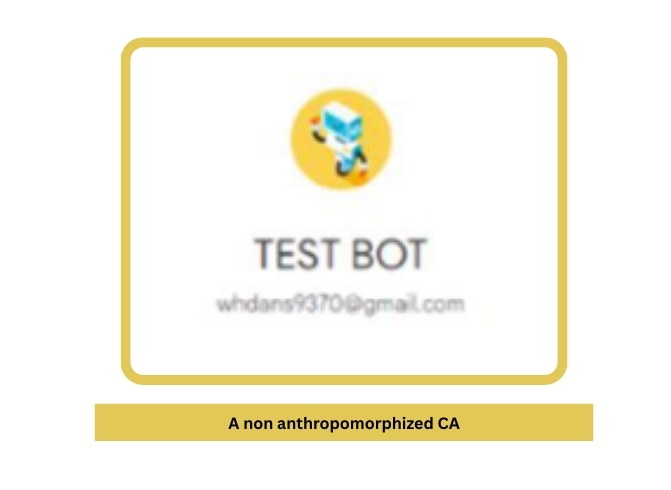
\includegraphics[width=0.31\textwidth]{Figures/12.jpg}
    \label{fig:ca_nonanthropomorphic}}
    \hfill
    \subfloat[]{%
    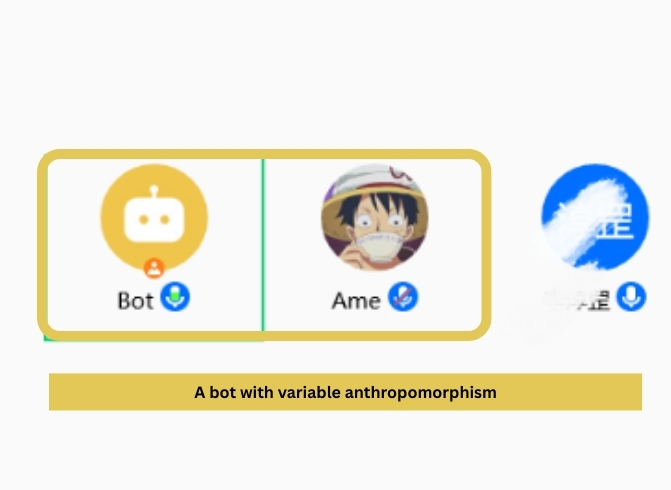
\includegraphics[width=0.31\textwidth]{Figures/14.jpg}
    \label{fig:ca_variable}}
    \hfill
    \subfloat[]{%
    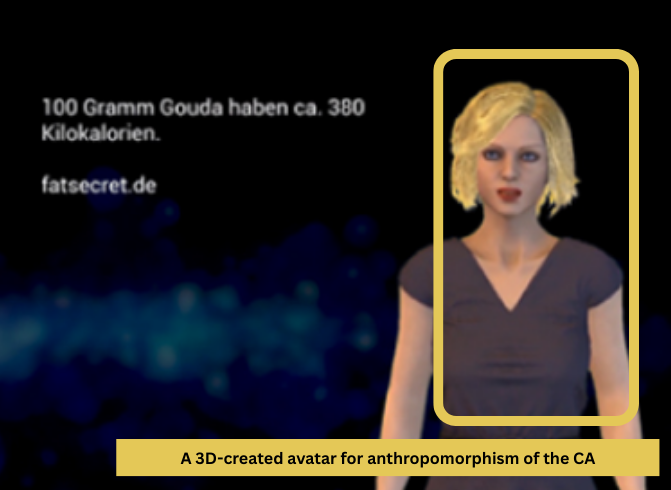
\includegraphics[width=0.31\textwidth]{Figures/13.png}
    \label{fig:ca_human}}
    \caption{\textbf{Anthropomorphism in conversational agents.}
    Examples show (a) a non-anthropomorphic CA, (b) a CA with selected
    anthropomorphic attributes, and (c) an anthropomorphized CA
    represented by a three-dimensional avatar.}
    \label{fig:CAs}
\end{figure*}

Different forms of anthropomorphism, as shown in Figure~\ref{fig:CAs}, can influence how users receive and evaluate information from a CA. Behavioral attributes affect how information is communicated during an interaction, whereas representational attributes affect how users perceive the identity and role of its source. Research on human--CA interaction consequently calls for closer attention to user groups, CA roles, interaction tasks, and the social conditions under which users receive generated information \parencite{jiang_humanai_2024}.

Existing studies show that these design attributes can affect information-system outcomes. For example, internal cues such as cognitive and emotional empathy and external cues such as virtual appearance can influence satisfaction with intelligent customer-service bots \parencite{hu_joint_2023}. Conversely, limited transparency and incomprehensible information can reduce trust in AI-generated advice and discourage users from adopting that advice \parencite{zhu_not_2023}. Algorithm acceptance also varies according to the task, users' expertise, and methodological conditions \parencite{kaufmann_task_2023}. These findings indicate that the effects of anthropomorphism cannot be separated from users' assessment and use of the information provided by a CA.

However, empirical findings remain mixed. Anthropomorphic attributes have been associated with greater user acceptance, engagement, trust, and social presence \parencite{ashfaq2020deploying,blut2021understanding,gong_how_2008,konya2023anthropomorphism,raamkumar2022empathetic}. Other studies report that human-like cues create unrealistic expectations, increase blame following service failures, produce feelings of eeriness, or reduce compliance when personalization appears intrusive \parencite{ciechanowski2019shades,clavel2015sentiment,crolic2022blame,chen_you_2021}. The same broad design strategy can therefore support information use in one setting while impairing users' judgments or expectations in another. Without estimates for specific attributes and outcomes, researchers and practitioners cannot determine whether these studies contradict one another or examine different forms of anthropomorphism under different conditions.

Prior reviews provide nascent guidance toward addressing this problem. \textcite{chaves2021should} identified social characteristics that apply generally to human--CA interaction and others whose effects depend on the application domain. \textcite{klein_effects_2025} synthesized 142 studies of human-like social cues in text-based CAs and reported a small-to-medium overall effect on social responses. However, existing reviews do not provide a detailed comparison between behavioral and representational attributes or systematically map individual attributes to user outcomes such as trust, information acceptance, learning, satisfaction, and interaction behavior. We define user outcomes as users' perceptions, experiences, intentions, behaviors, and performance when interacting with a CA. The literature therefore lacks systematic evidence showing which anthropomorphic attributes affect particular user outcomes and the magnitude of those effects.

We address this gap through the following research question:

\begin{quote}
\textit{How do anthropomorphic attributes of conversational agents affect user outcomes?}
\end{quote}

We examine this question using 583 effects extracted from 79 empirical articles published between 2018 and 2025. Of these, 169 effects from 23 studies contained sufficient statistical information for a three-level random-effects meta-analysis ($N$ = 21,104). We analyzed a further 373 non-calculable effects using vote counting, Fisher's combined probability test, and Stouffer's Z-score method. The combined analyses use 542 of the 583 extracted effects. This approach follows the role of meta-analysis in information-management research by synthesizing inconsistent findings, estimating benchmark effects, and identifying conditions under which relationships differ \parencite{mou_cohen_2024}.

This study makes four contributions. First, we derive a taxonomy that distinguishes behavioral attributes from representational attributes based on their co-occurrence in the 79-article corpus. Second, we estimate the overall effect of anthropomorphic design while accounting for the dependence of multiple effects reported within the same study. The three-level model produces a pooled Hedges' $g$ of 0.68, while correction for publication bias reduces the estimate to $g$ = 0.48. Third, we show that anthropomorphic attributes do not affect all user outcomes equally. Communication style ($g$ = 1.15) and personality traits ($g$ = 1.07) yield the largest attribute-level effects, whereas UX, trust, and learning exhibit moderate-to-large outcome-level effects. Fourth, we translate these results into guidelines for designing and managing CAs as information interfaces. Because publication bias is present and heterogeneity is considerable, the reported estimates should be interpreted as upper bounds instead of universal effects.

\section{Related Work}

% --- Section 2.1: Broad IS Context (Preserved your original text) ---
\subsection{Brief History of Conversational Agents}
CAs have existed for decades, since at least Weizenbaum's \texttt{ELIZA} in 1966, which simulated a psychotherapist \parencite{weizenbaum_elizacomputer_1966}\footnote{Before that, Alan Turing had discussed the prospect of a machine imitating humans in conversations in his seminal article from 1950 \parencite{turing_computing_1950}.}. Despite having been studied for decades, only the LLM technology has brought about a decisive breakthrough in the abilities of CAs to carry out conversations with human users. \textcite{peter_benefits_2025} use the term ``anthropomorphic conversational agents'' to characterize recent LLMs that, despite lacking genuine social understanding, excel at simulating empathy and persuasion to a degree that renders them nearly indistinguishable from real people. %Now, even though CAs have been studied extensively in fields like HCI and NLP, investigating anthropomorphism or ``human-likeness'' as a means to improve user engagement with CAs deviates from most earlier IS user engagement research, which has largely centered on the functional or instrumental value of information technology \cite{chandra_be_2022}. For this reason, it is worthwhile to discuss the nature of CAs as forms of IS.

Overall, %CAs function as interactive UIs that collect, process, and disseminate information through natural language \cite{nguyen2024conversational,mariani2023artificial,pfeuffer2019anthropomorphic}.
% Because natural language can be either written or spoken, CAs communicate with users through text, speech, or a combination of both \cite{diederich_conversational_2019}. 
% Furthermore, 
CAs can be categorized into (1) text-based CAs (written text only, no embodiment\footnote{Embodiment refers to the physical or visual representation of a CA, such as an avatar or robot body. While embodiment is one possible anthropomorphic attribute, anthropomorphism is a broader concept encompassing any human-like characteristic, including name, personality, communication style, and behavior.}), (2) virtual CAs (written and spoken interaction with virtual interactive avatars), (3) speech-based CAs (spoken interaction without embodiment), and (4) physical CAs (spoken interaction with physical embodiment) \parencite{diederich_design_2022}. 
Across these CA types, a shared trait is the reliance on natural language for interaction \parencite{diederich_design_2022}. 

Another key trait of CAs is that, unlike navigation-based UIs, CAs adapt to user needs \parencite{folstad2017chatbots,jain2018evaluating}. For example, a student can ask a CA for steps to solve a mathematics problem, and the CA will provide them. A CA can take multiple forms, including static or interactive virtual avatars, physical embodiments, or a disembodied form based solely on natural language \parencite{diederich_conversational_2019,diederich_design_2022}. These different implementations shape how users perceive CAs \parencite{peter_benefits_2025}, while making systems and information more accessible. \textcite{peter_benefits_2025} even argues that one of the core objectives of computer science is ``to make computers more accessible and more natural to interact with, \textit{by making computing more human-like}'' (p. 1, emphasis by us). \textcite{chaves2021should} further emphasizes the role of interaction design by postulating that ``making a conversational agent acceptable to users is primarily a social, not only technical, problem'' (p. 729). These conceptual underpinnings have prompted researchers to theorize about anthropomorphism in computer systems and CAs, in particular.

% To this end, modern CAs are widely diffused. They integrate both with enterprise and consumer IS, including customer relationship management (CRM) systems and knowledge management platforms \cite{mariani2023artificial}, technical support, customer service, and social media \cite{diederich_design_2022,schuetzler_impact_2020}, among other types of IS. While CAs were historically viewed as passive retrieval tools, modern CAs, enabled by LLMs, not only fetch information but can also interpret it, making them active agents in the information flow from systems to users \cite{allouch2021conversational}. 
% % --- Added Transition to Anthropomorphism ---
% However, as CAs take on these active roles, the distinction between ``system'' and ``social actor'' blurs. This shift calls for a deeper understanding of how the design of the CA itself, through its humanization, impacts the interaction between the user and the system.

\subsection{Theories of Anthropomorphism in Software Systems}

%Anthropomorphism, the attribution of human characteristics, emotions, or behaviors to non-human entities, draws on the CASA paradigm, which posits that users unconsciously apply social rules to technology \cite{nass1994computers}. Anthropomorphism is a critical component in CAs, because ``[user] engagement [with CAs] depends, in turn, on conversational AI’s similarity, or likeness to the human beings it is intended to replace'' \cite{chandra_be_2022} (p. 969).

The theoretical foundation for understanding why users respond socially to CAs can be derived from the ``\textbf{C}omputers \textbf{A}re \textbf{S}ocial \textbf{A}ctors'' (CASA) paradigm \parencite{nass2000researching,nass1994computers}. Introduced by \textcite{nass1994computers}, CASA argues that humans apply social rules to computers even when they know they are interacting with machines. The key insight is that social responses to computers ``are automatic and
unconscious'' (p. 77) \parencite{nass1994computers}. When computers display social cues such as language or voice, users automatically apply human interaction behaviors that include, for example, (1) gender stereotyping (e.g., rating female-voiced computers as more knowledgeable about relationships), (2) reciprocity (e.g., feeling obliged to help a computer that provided assistance), and (3) politeness norms (e.g., giving more favorable evaluations when the computer itself asks for feedback) \parencite{nass1997machines}. 

A related concept is \textit{social presence}, which refers to ``the degree of salience of the other person in the interaction'' (p. 65) \parencite{short1976social}. In the CA context, social presence reflects the extent to which users perceive the agent as a real social entity instead of merely a tool \parencite{oh2018systematic}. While CASA explains the automatic process of applying social rules, social presence addresses the sense of interacting with another being. Social presence is associated with increased trust and engagement \parencite{gunawardena1995social}. Prior research \parencite{gambino2020building,koger2023casa} %raises questions about whether CASA effects persist as users become familiar with technology. Gambino et al. \cite{gambino2020building} proposed extending CASA, arguing that users may develop distinct human-media scripts over time. Furthermore, a replication study found that participants no longer responded socially to desktop computers after 30 years of exposure \cite{koger2023casa}. This 
suggests that CASA effects may wane over time and be strongest for emerging technologies, such as LLM-based CAs. CASA also implies that even minimal anthropomorphic cues can trigger social responses. For example, \textcite{araujo2018living} showed that simply assigning a name to the CA can increase users' perception of the agent's human-likeness. Therefore, the question is not whether to anthropomorphize or not, but \textit{how}.  %, thus motivating RQ1 and RQ2. These aspects have thus far eluded mainstream research in IS; as eloquently put by Peter et al., while much research attention is given to improving LLMs' reasoning capabilities, ``the progress in communicative abilities remains underappreciated'' (p. 1).

% This temporal contingency matters for interpreting our findings.  The studies in our corpus examine LLM-based CAs, for which CASA  effects may be stronger than for legacy systems. Our findings are  therefore consistent with CASA predictions instead of a test of its underlying mechanisms.

Research on embodied and voice-based CAs establishes that anthropomorphic effects extend well beyond what text-centric studies can capture. Coordinated verbal and nonverbal cues, relational consistency across sessions, embodied social signals such as gaze and gesture, and voice para-linguistics each affect social agency, trust, and presence in ways that text-based behavioral attributes alone cannot replicate \parencite{cassell2000embodied,bickmore2005relational,kramer2003socially,clark2019makes}. This literature is not represented in our empirical corpus, which is predominantly text-centric. 
% Thus the design guidelines, each with 5 profile sentences, therefore not be extended to embodied or voice agents without further empirical grounding. 

% --- Section 2.2: Focus on Attributes & Effects (Aligns with RQ1) ---

%\subsection{Different Attributes for Anthropomorphism}



% --- Section 2.3: Focus on Implementation (Aligns with RQ2) ---
%\subsection{Technical Implementation and Persona Consistency}
\subsection{The Empirical Effects of Anthropomorphism on Users}
%Implementing anthropomorphism in CAs involves decisions spanning three areas: how anthropomorphic attributes are represented, how consistency is maintained, and how the system adapts to users.

% \textit{Anthropomorphic attribute representation} refers to how human-like attributes are encoded in the system. Early approaches used explicit profile descriptions---structured lists of attributes such as hobbies, occupation, and preferences---that condition the CA's responses \cite{zhang2018personalizing}. The PersonaChat dataset exemplifies this approach, providing 1,155 personas with 5 profile sentences each for training dialogue systems. Alternative approaches embed persona implicitly through fine-tuning on character-specific dialogue \cite{shuster2019dialogue} or through prompt engineering with LLMs \cite{jandaghi2023faithful}. The choice between explicit and implicit representation affects both development effort and the degree of control designers have over the CA's expressed identity.

% \textit{Persona consistency} is the ability of a CA to maintain a stable identity without contradicting itself across turns or sessions. This remains a primary technical challenge \cite{song2020generating}. A CA that claims to be a doctor in one turn but discusses its experience as a teacher in another violates consistency and may reduce user trust. Technical solutions include natural language inference models that verify alignment between utterances and persona profiles \cite{welleck2019dialogue}, reinforcement learning approaches that optimize for coherence \cite{song2021bob}, and memory mechanisms that track what the CA has previously stated \cite{xu2022beyond}. Evaluations show that even state-of-the-art LLMs struggle to maintain consistent personas in extended conversations \cite{maharana2024evaluating}, so although the fundamental challenge \cite{turing_computing_1950} of the AI ``remembering'' and recalling parts of the conversation has been resolved to a great extent, CAs can still exhibit traces of this problem.

% \textit{Persona adaptability} concerns whether the CA adjusts its characteristics based on user input or context. Fixed personas maintain the same attributes throughout interaction, while adaptive personas modify their behavior in response to user preferences, emotional state, or conversational history \cite{huang2023personalized}. Adaptive approaches can increase perceived personalization but risk inconsistency if changes are not managed coherently. Memory-augmented architectures address this by maintaining long-term user models that inform persona expression without contradicting core identity attributes \cite{xu2022beyond,zhong_memorybank_2024}.


%\subsection{User Outcomes of CA Anthropomorphization}
Research on anthropomorphic CAs examines various user outcomes, yet these findings remain scattered across studies. Studies report effects on constructs such as trust \parencite{nordheim2019trust}, satisfaction \parencite{haugeland_understanding_2022}, engagement \parencite{mehra_chatbot_2021}, and learning \parencite{zheldibayeva_genai_2025}, showing that %, but there is no clear understanding of what types of outcomes anthropomorphization actually affects.
%Research shows that 
anthropomorphism affects user outcomes %\cite{pfeuffer2019anthropomorphic,adam2021ai} 
through perceiving the agent as a ``real'' social entity instead of a ``tool'' \parencite{meyer2023leverage,wang2021seeing}. For example, anthropomorphism in customer service CAs increases engagement and purchase intentions \parencite{depaula2025anthropomorphism,luo2019frontiers}. Researchers have also found that CAs' anthropomorphism increases perceptions of competence and warmth, which in turn support empathy and increase users' willingness to adopt CAs \parencite{kim_what_2024}. \textcite{rapp_human_2021} note that ``[the] perception of humanness may increase the willingness to establish a common ground between the chatbot and the user and to express more sociable desirable traits, as well as intimacy and closeness''.

However, excessive human-likeness can trigger the \textit{uncanny valley} effect, in which the CA resembles a human too closely, causing feelings of eeriness \parencite{mori_bukimi_1970,soni2024chatbot}. Furthermore, mismatches between human-like cues and a CA's actual capabilities lead to expectancy violations that undermine satisfaction more severely than purely functional failures (i.e., when a system's functionality fails) \parencite{ischen2024communication,qu2024chatbot}. Other commonly mentioned challenges in CA design include a lack of conversational abilities and unappealing appearance \parencite{diederich_design_2022}, as well as the risk of manipulation \parencite{chaves2021should}.

Overall, the empirical findings on the effects of anthropomorphism are scattered and mixed, such that anthropomorphism improves outcomes in some studies \parencite{go2019humanizing} but produces negative effects in others \parencite{crolic2022blame}. For example, anthropomorphic design may increase trust \parencite{go2019humanizing,konya2023anthropomorphism}, yet decrease compliance when users find personalization intrusive \parencite{chen_you_2021}. Some studies report that anthropomorphism improves user outcomes, while others find no or negative effects. Without a systematic analysis of which specific anthropomorphic attributes produce these different outcomes, we cannot determine whether studies genuinely contradict each other or whether different attributes simply affect users in distinct ways.

Previous reviews have examined anthropomorphism's effects on specific outcomes, such as trust \parencite{bach2024systematic}, or focused on technical implementation \parencite{chen2024trends}, but the field lacks the ``bigger picture'' of the empirical consequences of the \textit{anthropomorphic design} of CAs. A systematic review by \textcite{rapp_human_2021} identified it being ``evident that literature lacks design related research. There are no studies that seriously tackle [CA] design issues.'' While \textcite{klein_effects_2025} meta-analysis established that human-like social cues in text-based agents produce positive effects, this work did not distinguish between behavioral and demographic attributes, examine multi-modal agents, or analyze the relationship between attributes and specific user outcomes. This study examines the effects of specific behavioral and demographic attributes on user outcomes within this predominantly text-centric corpus.

\section{Methodology}
This meta-analysis examined the impact of anthropomorphic attributes in CAs on user outcomes. We synthesized empirical findings from a systematic literature review \parencite{amin2025anthropomorphism} of 79 articles published between 2018 and 2025, employing a two-track approach to maximize data utilization. Of the 583 extracted effects, 169 (30.4\%) contained sufficient statistical information for effect size computation and were analyzed using a random-effects meta-analysis. The remaining 373 effects (69.6\%) reported directional findings and significance indicators but lacked the statistical detail necessary to calculate effect sizes. Discarding these effects entirely would have excluded the majority of the extracted evidence, so we applied three complementary synthesis methods to incorporate this directional evidence without requiring exact effect size estimates.

\subsection{Systematic Literature Review}

We conducted searches following the PRISMA guidelines \parencite{page_prisma_2021} in four academic databases: SCOPUS, Web of Science, IEEE Xplore, and ACM Digital Library. The search string combined CA terminology (``conversational agent*,'' ``chatbot*,'' ``virtual agent*,'' ``dialogue system*'') with anthropomorphism (``anthropomorph*,'' ``human-like,'' ``persona*,'' ``personality,'' ``gender,'' \newline``avatar''). Keywords were finalized through three pilot searches: initial broad terms were iteratively narrowed based on title-level precision, and anthropomorphism-specific terms were added after the first round retrieved insufficient empirical CA studies. We limited our search to English-language, peer-reviewed articles published between January 2018 and August 2025, capturing the state of the art in CAs \parencite{zhang2018personalizing}. % when neural language models became widespread.

The principal investigator (PI) screened 735 identified articles in two stages. First, the PI reviewed the titles and abstracts against predefined inclusion criteria, resulting in 312 potentially relevant articles. Second, the PI reviewed the full texts against the same inclusion criteria and recorded the reasons for exclusion for each rejected article. A random sample of 10\% of full-text decisions was cross-checked by a second author to verify consistency, with disagreements resolved through discussion. Studies were included if they: (1) reported empirical quantitative data; (2) examined user interactions with a CA; (3) manipulated or measured at least one anthropomorphic attribute; and (4) measured a user outcome. Studies were excluded if they: (1) were purely technical without user evaluation; (2) were qualitative-only; (3) were reviews or meta-analyses; or (4) examined physical robots without a conversational interface.

The PI excluded purely technical studies without user evaluation, qualitative-only studies, reviews, and studies of physical robots without conversational interfaces. Qualitative-only studies were excluded as primary sources because they do not report the statistical information necessary to compute effect sizes.  Implementation quality was not used as an exclusion criterion at the screening stage; rather, quality issues were addressed at the effect extraction stage by removing individual effects with impossible values or insufficient sample sizes (see Section~3.5). No studies were excluded solely on the basis of implementation quality, ensuring that the corpus reflects the full range of empirical work on anthropomorphic CA design. This process yielded 79 empirical studies that comprise our final corpus.

\subsection{Effect Extraction and Coding}

Five trained coders extracted effects from the 79 articles using a standardized protocol (see the online appendix\footnote{\href{https://osf.io/7rj6f/overview?view_only=35b327583fee4222b5b336465107580c}{https://bit.ly/4nn1NhZ}} for details), with 10\% of the articles being double-coded to ensure reliability. Instead of extracting generic study characteristics, we identified and coded individual effects representing relationships between anthropomorphic attributes (as independent variables) and specific user outcomes (as dependent variables) within each study. Inter-coder reliability among five coders for effect extraction was substantial (Fleiss' $\kappa$ = 0.81). Coding was inductive as coders generated categories from the data instead of applying a predefined codebook, with the final category scheme emerging through iterative discussion within the coding team. A full mapping of included studies to anthropomorphic attributes, study designs, outcome measures, and main effects is provided in Table~A1 of the online appendix.
% This granular approach treats each attribute-outcome relationship as an independent observation, recognizing that single studies often examine multiple anthropomorphic attributes and measure various outcomes.

From the 79 articles, we extracted 583 distinct effects. Each effect captured a reported relationship between an anthropomorphic implementation and a user outcome, along with available statistical information. For each effect, coders recorded the specific anthropomorphic attribute manipulated or measured, the outcome variable assessed, the direction of the relationship (positive, negative, or null), and any available statistical information, including means, standard deviations, test statistics, effect sizes, and p-values. This extraction of the effect level enables more precise analysis than aggregation at the study level, as it preserves the specific combinations of attributes and results that comprise our research question.

Of the 583 extracted effects, 177 (30.4\%) contained effect size calculations, which are referred to as calculable effects in the remainder of the work. Of these, 8 were removed due to quality issues; specifically, impossible effect size values (e.g., r $>$ 1.0) or sample sizes insufficient for stable estimation (n $<$ 10), leaving 169 calculable effects. The other 406 effects (69.6\%) provided directional information and significance indicators but lacked effect-size details. We refer to them as non-calculable effects throughout the remainder of the work. For these, we removed 33 effects due to missing information, leaving 373 non-calculable effects. 

For calculable effects, we employed a three-level random-effects model as the primary analysis and the DerSimonian-Laird two-level model for subgroup comparisons, whereas voting methods were applied to non-calculable effects.

\subsection{Categorization of Anthropomorphism}

To investigate which anthropomorphic attributes affect user outcomes, we categorized the attributes implemented across studies. To this end, we employed hierarchical agglomerative clustering (see the online appendix for details). First, we extracted 73 unique attribute types across the 79 studies (see Table \ref{tab:attr-dist} for category distributions; the complete list of all 73 attributes is provided in Table~A2 of the online appendix)
types across the 79 studies and analyzed their co-occurrence patterns, which attributes researchers implemented together, using Jaccard similarity coefficients with Ward's linkage criterion. %This approach reveals natural groupings based on empirical implementation patterns instead of theoretical assumptions. 
Analysis of the resulting hierarchical agglomerative clustering identified two primary clusters at the optimal cut-off point as behavioral attributes that manifest through agent actions during interaction (communication style, personality traits, actions, emotional expressions) and demographic attributes representing relatively fixed aspects of CAs identity (demographic identity, roles, names, visual representations, voice characteristics). The two-cluster solution was selected based on the largest within-cluster Jaccard similarity drop in the dendrogram; a three-cluster solution was also examined, but produced one cluster ($n$ = 3) too small for meaningful analysis. Chi-square test confirmed that behavioral and demographic attributes have different prevalence rates across studies ($\chi^2$ = 8.47, p = .004), with behavioral attributes appearing in 65.5\% of studies compared to 38.8\% for demographic attributes. Detailed clustering methodology and complete attribute listings are available in the online supplementary material.

% \begin{table}[t]
% \centering
% \caption{\textbf{Distribution of anthropomorphic attribute categories in 79 anthropomorphization studies.} Behavioral anthropomorphization is more frequent. }
% \footnotesize
% \label{tab:attr-dist}
% \begin{tabularx}{\textwidth}{@{}llccX@{}}
% \toprule
% \textbf{Main category} & \textbf{Sub category} & \textbf{n} & \textbf{\%} & \textbf{Attributes Applied} \\
% \midrule
% \multirow{3}{*}{\shortstack[l]{Behavioral\\attributes\\(n = 76, 62.8\%)}} & Communication style & 29 & 24.0 & conversational (n = 8), polite (n = 2), professional (n = 2) \\
% & Personality traits & 28 & 23.1 & empathetic (n = 4), helpful (n = 3), supportive (n = 3) \\
% & Actions & 19 & 15.7 & proactive (n = 2), initiative-taking (n = 2), engaging \\
% \midrule
% \multirow{3}{*}{\shortstack[l]{Demographics\\(n = 45, 37.2\%)}} & Demographic identity & 22 & 18.2 & gender (n = 11), age (n = 5), cultural background \\
% & Role/occupation & 14 & 11.6 & expert (n = 1), personal assistant (n = 1), tutor (n = 1) \\
% & Visual/physical appearance & 9 & 7.4 & character (n = 1), facial covering (n = 1), embodiment \\
% \bottomrule
% \end{tabularx}
% \end{table}

\begin{table}[t]
\centering
\caption{\textbf{Distribution of anthropomorphic attribute categories in 79 anthropomorphization studies.} Behavioral anthropomorphization is more frequent.}
\footnotesize
\label{tab:attr-dist}
\begin{tabular}{@{}p{4cm}p{5.4cm}rr@{}}
\toprule
\textbf{Category} & \textbf{Subcategory} & \textbf{n} & \textbf{\%} \\
\midrule
\multirow{3}{*}{\shortstack[l]{Behavioral\\(n=76,\\62.8\%)}} 
& Communication style & 29 & 24.0 \\
& Personality & 28 & 23.1 \\
& Actions & 19 & 15.7 \\
\midrule
\multirow{3}{*}{\shortstack[l]{Demographic\\(n=45,\\37.2\%)}} 
& Demographic identity & 22 & 18.2 \\
& Role/occupation & 14 & 11.6 \\
& Visual/appearance & 9 & 7.4 \\
\bottomrule
\end{tabular}
\vspace{0.5em}
\par\noindent\scriptsize
\textbf{Attributes Applied:} 
\textit{Behavioral}---Communication\ style: conversational (8), polite (2), professional (2); 
Personality: empathetic (4), helpful (3), supportive (3); 
Actions: proactive (2), initiative-taking (2), engaging. 
\textit{Demographics}---Demographic\ identity: gender (11), age (5), cultural background; 
Role/occupation: expert (1), personal assistant (1), tutor (1); 
Visual/appearance: character (1), facial covering (1), embodiment.
\end{table}

\subsection{Categorization of Outcome Variables}

The 583 effects represented relationships with diverse outcome measures ranging from subjective satisfaction to objective performance metrics. Two coders jointly conducted open coding to categorize measures based on their underlying constructs. This process involved assigning umbrella labels to specific variables (e.g., trust, competency, and reliability are combined under the category of `trust and credibility'). This was done collaboratively, with one coder suggesting a label and another coder verifying its logical compatibility with the specific variable. %, achieving 94\% agreement. 
Here, participant demographics reported in included studies, where available, including age, gender, and prior technology experience, were treated as moderators within the seventh category.
This process resulted in seven outcome categories (see Table \ref{tab:categories}). We used these categories to analyze whether anthropomorphic attributes produce consistent effects or particularly influence specific outcome types. %(1) \textit{UX and satisfaction} (measures of satisfaction, usability, enjoyment, interaction quality); (2) \textit{trust and credibility} (trust formation, reliability, willingness to rely on information); (3) \textit{learning and performance} (task accuracy, knowledge acquisition, problem-solving); (4) \textit{social perception and anthropomorphism} (perceived humanness, social presence, relationship quality); (5) \textit{behavioral and interaction patterns} (engagement duration, message frequency, compliance); (6) \textit{technology acceptance and adoption intentions} (behavioral intentions, adoption decisions); and (7) \textit{individual differences as moderators} (examining how user characteristics moderate effects). We used these categories to analyze whether anthropomorphic attributes produce consistent effects or particularly influence specific outcome types.

\begin{table}[h]
\caption{Categories of user outcome variables.}
\label{tab:categories}
\footnotesize
\begin{tabular}{@{}p{0.35\columnwidth}p{0.58\columnwidth}@{}}
\toprule
\textbf{Category} & \textbf{Variables contained} \\
\midrule
UX and satisfaction & Satisfaction, usability, enjoyment, interaction quality \\
\addlinespace
Trust and credibility & Trust formation, reliability, willingness to rely on information \\
\addlinespace
Learning and performance & Task accuracy, knowledge acquisition, problem-solving \\
\addlinespace
Social perception and anthropomorphism & Perceived humanness, social presence, relationship quality \\
\addlinespace
Behavioral and interaction patterns & Engagement duration, message frequency, compliance \\
\addlinespace
Technology acceptance and adoption intentions & Behavioral intentions, adoption decisions \\
\addlinespace
Individual differences as moderators & User characteristics \\
\bottomrule
\end{tabular}
\end{table}



\subsection{Effect Size and Meta-Analytic Procedures}

To synthesize the effects quantitatively, we converted diverse statistical metrics into a common metric, Hedges' g, with a small-sample correction. Hedges' $g$ effect size follows the interpretation used in \textcite{cohen2013statistical} guidelines, classifying the absolute values $\leq0.2$ as small, $>0.2$ to $\leq0.5$ as medium, $>0.5$ to $\leq0.8$ as large, and $>0.8$ as very large effects. The 177 effects with calculable statistics reported various formats: eta-squared (34.5\%), Pearson's r (16.9\%), Cohen's $d$ (15.3\%), F-statistics (9.0\%), Spearman's $\rho$ (6.8\%), chi-square (6.8\%), t-statistics (4.0\%), odds ratios (2.3\%), and other metrics (4.4\%). We applied established conversion formulas, carefully preserving the directions of effects. After data quality checks, removing effects with impossible values (e.g., standardized statistics outside feasible ranges) or sample sizes below n = 10, following established meta-analytic guidance \parencite{borenstein2010basic}, 169 effects from 23 studies ($N$ = 21,104 participants) were included in the meta-analysis.

We employed a three-level random-effects model \parencite{vanden2013three} as the primary analysis, partitioning variance into within-study (Level 2) and between-study (Level 3) components via restricted maximum likelihood (REML) estimation. This model accounts for the nested structure of multiple effects within studies, which is appropriate given a mean of 7.3 effects per article. The DerSimonian-Laird two-level model \parencite{dersimonian1986meta} was retained for subgroup analyses and as a comparison estimate. Heterogeneity was assessed using $Q$-statistics, $I^2$, and 95\% prediction intervals.

To examine whether attribute type and outcome category moderated effect sizes, we conducted subgroup analyses partitioning $Q_{\text{total}}$ into $Q_{\text{between}}$ and $Q_{\text{within}}$, and formal weighted least-squares meta-regression testing each moderator with an omnibus $Q_{\text{model}}$ statistic and $R^2$ analog indicating variance explained.
Finally, publication bias was assessed using Egger's regression test \parencite{egger1997bias} and Duval and Tweedie's iterative trim-and-fill procedure \parencite{duval2000trim}, which estimates and imputes missing studies to produce a bias-adjusted pooled effect. Fail-safe $N$ \parencite{rosenthal1979file} is also reported for comparability with prior meta-analyses, though trim-and-fill is the primary correction given the well-documented limitations of fail-safe $N$ under high heterogeneity \parencite{page2024missingevidence}.

\subsection{Methods for Non-Calculable Effects}

The 406 effects that lack calculable effect sizes still provided directional and significance information. To maximize data utilization and strengthen our answer to the research question, we used three complementary synthesis methods that incorporate this evidence without requiring exact effect-size estimates.

First, we used \textit{vote counting} to categorize each effect as positive, negative, or null based on reported findings. We then tested whether positive effects occurred more frequently than expected by chance using \textit{binomial tests}. If anthropomorphic attributes consistently improve user outcomes, positive effects should substantially outweigh adverse effects. This method provides evidence on the overall effect direction across the entire dataset, including studies with insufficient statistics for meta-analysis. 

Second, for the 269 effects reporting significance tests, we used \textit{Fisher's combined probability test} \parencite{fisher1932statistical} on the aggregated p-values using the formula $\chi^2 = -2\sum_{i=1}^{k} \ln(p_i)$ with df = 2k. When exact p-values were not available, we substituted p = 0.025 for effects reported as significant (p $<$ 0.05) and p = 0.50 for non-significant effects. Although this substitution introduces uncertainty, it allows the inclusion of studies that lack precise p-values, thereby testing the overall pattern of statistical significance. % deviates from chance. %, providing independent confirmation of the results of quantitative meta-analysis.

Third, we used Stouffer's Z-score method \parencite{whitlock2005combining} to combine standardized effect directions using $Z_{combined} = \frac{\sum_{i=1}^{k} Z_i}{\sqrt{k}}$, weighting all studies equally while incorporating direction. This approach leverages information on significance and direction when exact magnitudes are unavailable \parencite{whitlock2005combining}.
We applied all three methods to behavioral versus demographic attributes, and for each outcome category, we achieved a comprehensive synthesis that addressed our research question across multiple types of evidence using both  %The convergence or divergence of findings across quantitative meta-analysis, vote counting, Fisher's test, and Stouffer's Z-score reveals the robustness of conclusions. 
non-calculable (n = 373) and calculable effects (n = 169), making a total of 542 of 583 recorded effects (93.0\% data utilization). 

\section{Results}

Our RQ asks how anthropomorphic attributes of CAs affect user outcomes. Across the different analyses, anthropomorphic design was generally associated with better user outcomes, but the strength of this relationship depended on the attribute implemented and the outcome measured. We first report the overall relationship, followed by the results for specific attributes, outcome categories, and attribute--outcome combinations.

\subsection{Overall Effects}

The three-level REML model, which partitions variance into within-study ($\hat{\sigma}^2_v$ = 0.695) and between-study ($\hat{\tau}^2$ = 0.356) components, yielded a pooled Hedges' $g$ = 0.68 (95\% CI [0.38, 0.98], $p$ $<$, .001) which is the primary estimate. The two-level DerSimonian-Laird model yielded $g$ = 0.73 (95\% CI [0.59, 0.87]). This two-level estimate is inflated by effect dependence and should not be treated as the benchmark in isolation. Heterogeneity was considerable ($I^2$ = 90.4\% total, with 59.7\% within-study and 30.6\% between-study). The 95\% prediction interval [$-$0.97, 2.43] indicates that a new study could produce an effect ranging from negligible negative to large positive, confirming that the grand mean does not represent a reliable benchmark for any individual context. This variability motivated our subsequent analyses examining which specific attributes and outcomes drive these effects.

Including multiple effects from the same study ($M$ = 7.3 effects per article) introduces dependence. A one-effect-per-study sensitivity analysis (averaging effects within each study) yielded $g$ = 0.64 (95\% CI [0.36, 0.91]), a 14.8\% reduction relative to the two-level estimate. Both the three-level and one-per-study estimates are reported alongside the two-level estimate throughout. All three indicate moderate positive effects with overlapping confidence intervals, confirming the direction and practical significance of the finding.

\subsection{Behavioral and Demographic Attributes} \label{sec:beh}

Effect sizes differed significantly across attribute subgroups ($Q_{\text{between}}$(3) = 193.45, $p$ $<$ .001; see Figure \ref{fig:attributes}). Behavioral attributes, including polite versus impolite language, socially oriented versus task-oriented voice feedback, proactive dialogue actions, and repair strategies, resulted $g$ = 0.75 (95\% CI [0.57, 0.94], $k$ = 89). Representational attributes such as voice, gender, assigned demographic identity, visual avatars, and human names produced $g$ = 0.70 (95\% CI [0.33, 1.06], $k$ = 42).\footnote{These categories comprise 131 of 169 effects. The remaining 38 examined contextual factors ($k$ = 26) and user moderators ($k$ = 12) were analyzed separately.} The magnitude difference between behavioral and representational attributes is small (0.05), and formal meta-regression found no significant difference between attribute types ($Q_{\text{model}}$(3) = 0.61, $p$ = .894). Practitioners should not de-prioritize representational design solely on the basis of this comparison.

Among behavioral attributes, communication style had the largest effect, $g$ = 1.15, 95\% CI [0.72, 1.59], $k$ = 25. CAs employing natural conversational patterns, contextually-appropriate formality levels (formal versus informal language), and adaptive politeness strategies (polite versus non-polite phrasing) generated effects exceeding one standard deviation. Personality traits produced the 
second largest effects, $g$ = 1.07, 95\% CI [0.54, 1.59], $k$ = 19, indicating that personality traits (i.e., extroversion, agreeableness, and openness) improve user outcomes.

Among representational attributes, visual appearance, $g$ = 0.82, 95\% CI [0.19, 1.45], $k$ = 23, produced stronger effects than demographic identity assignments, $g$ = 0.52, 95\% CI [0.27, 0.77], $k$ = 15. We further analyzed the data and found that voice gender (male versus female) had minimal effects (mean $g$ = 0.26, $k$ = 5), whereas language status (low-status versus high-status) had larger effects (mean $g$ = 1.21, $k$ = 5). Both estimates rest on five effects and should be treated as preliminary.

\begin{figure}
    \centering
    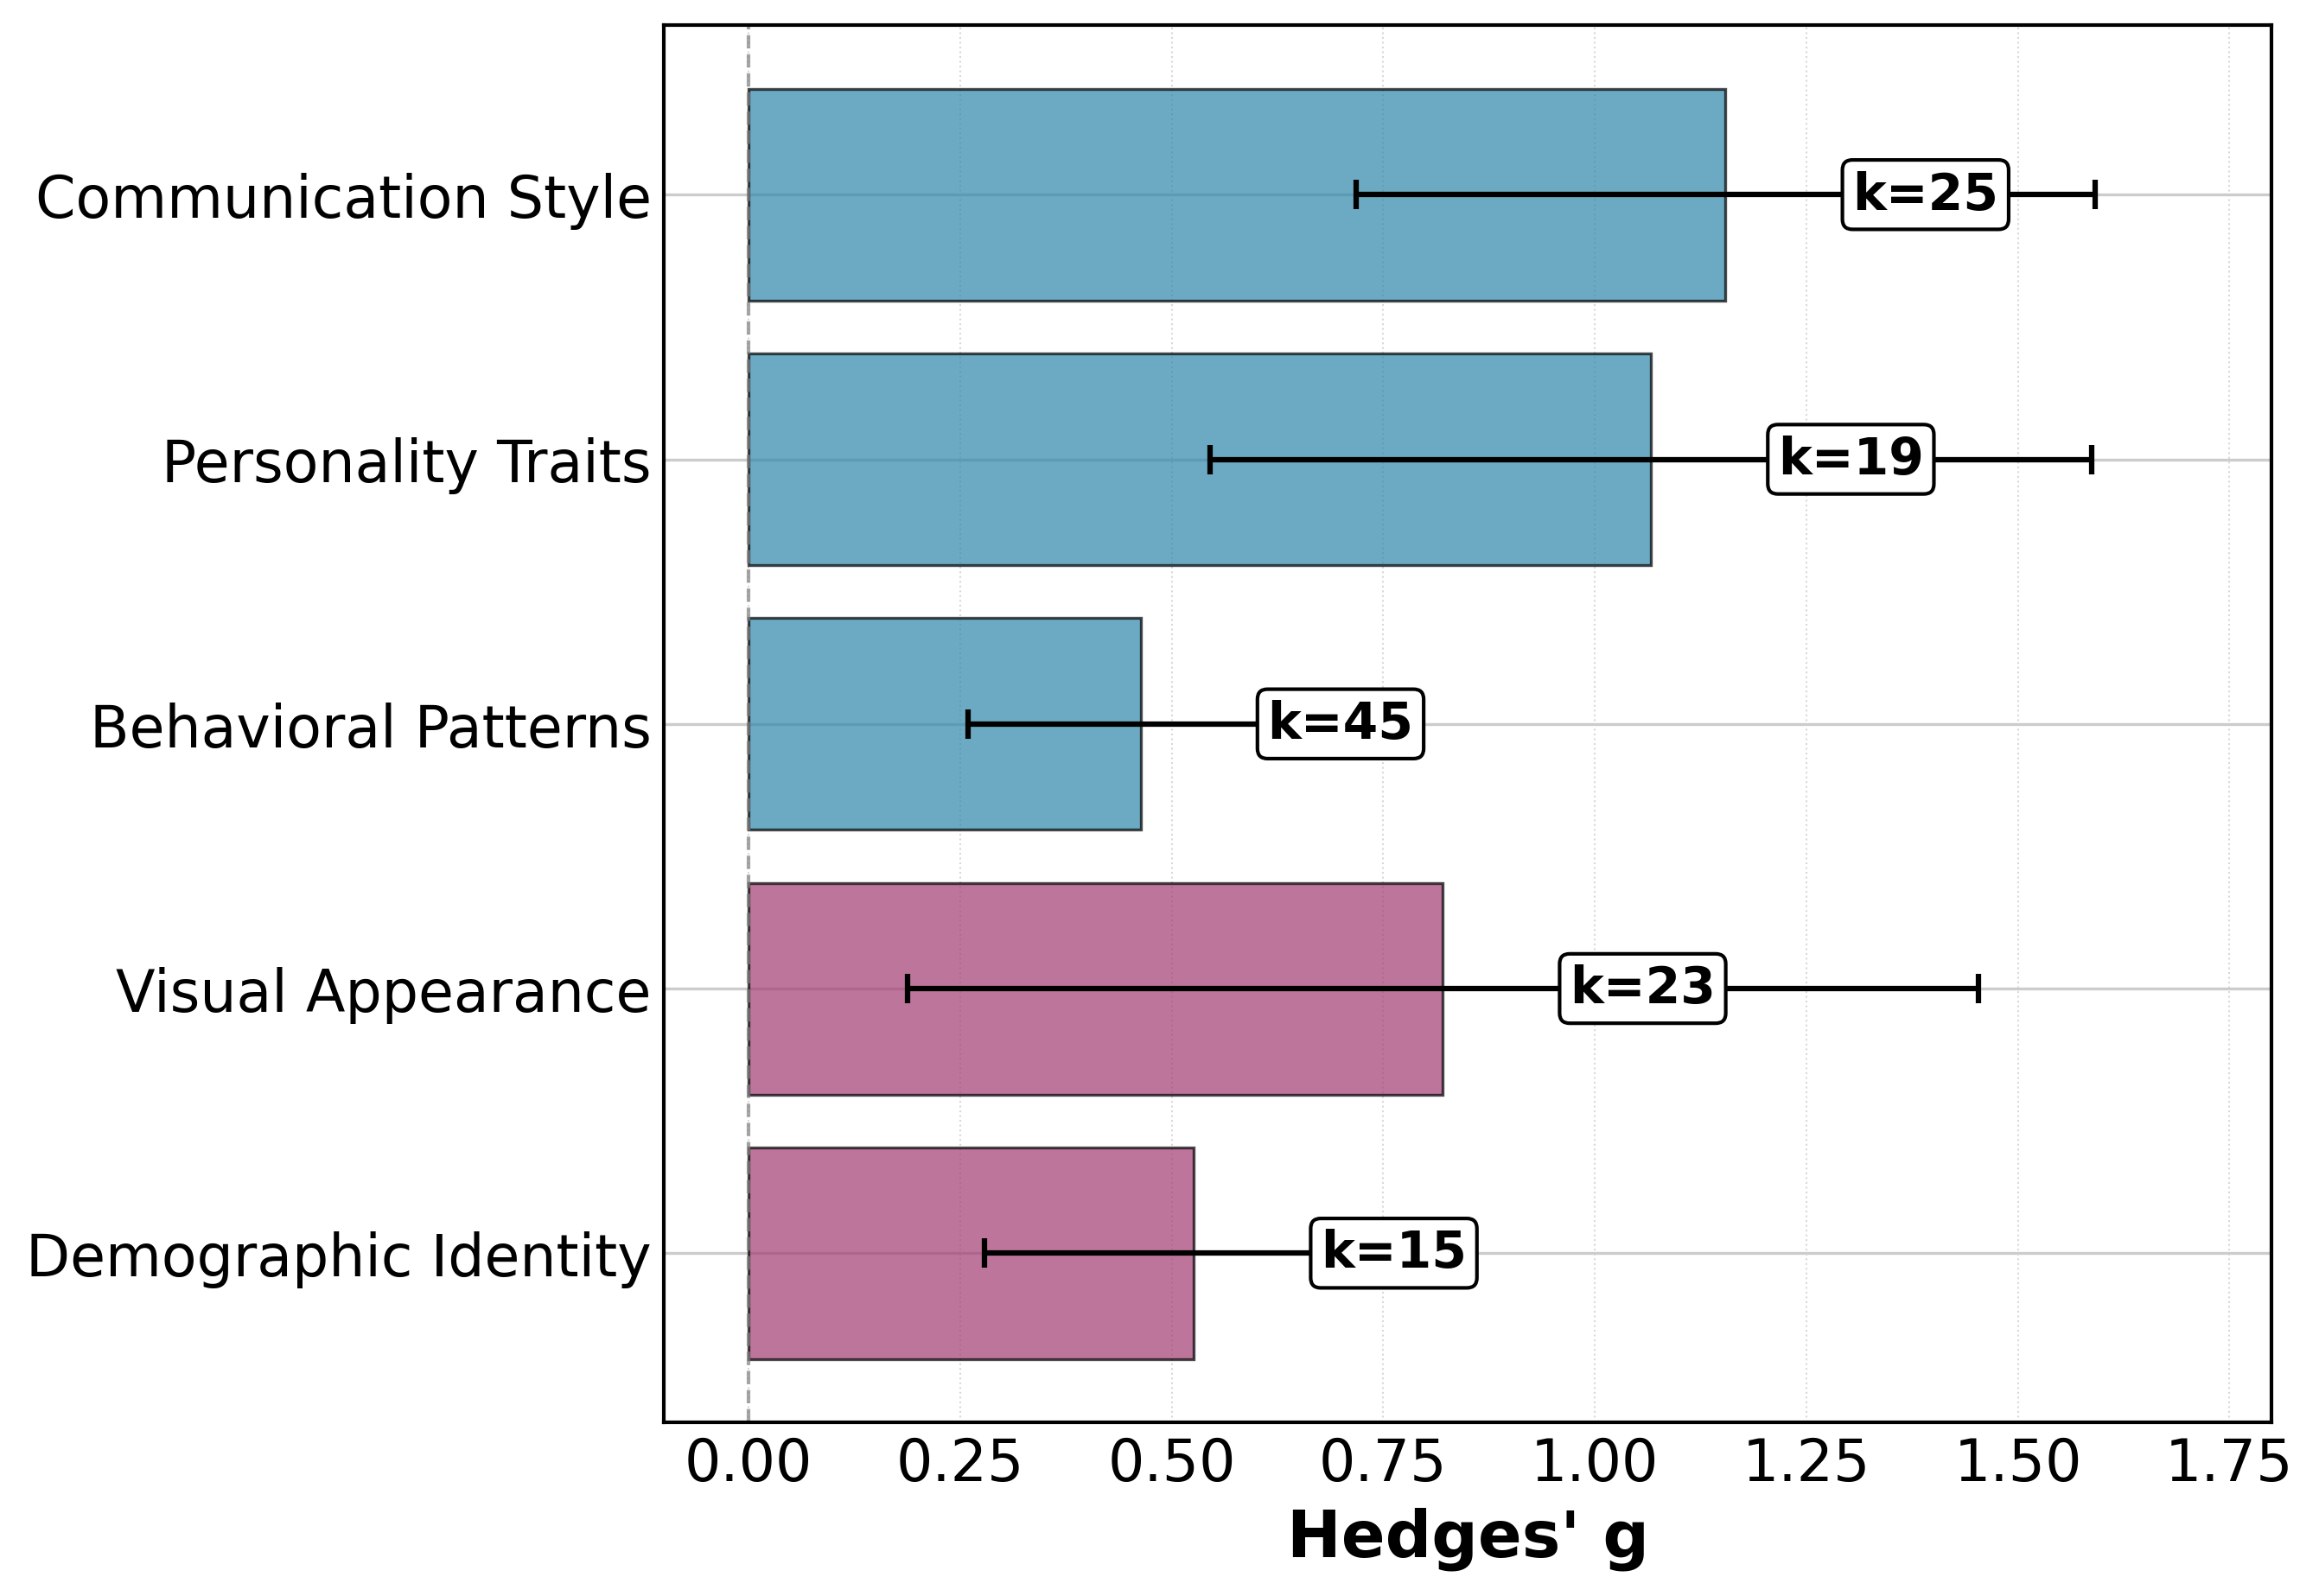
\includegraphics[width=0.6\linewidth]{Figures/figure2a_subcategories.png}
    \caption{Effect sizes for behavioral and demographic attributes 
    for anthropomorphism.}
    \label{fig:attributes}
\end{figure}

\subsection{Effects by Outcome Type} \label{sec:out}

Anthropomorphic attributes affected outcomes differently across measurements. The analysis across outcome categories showed systematic variation ($Q_{\text{between}}$(6) = 169.80, $p$ $<$ .001), indicating that different attributes have different effect sizes.

UX outcomes showed large effects ($g$ = 0.69, 95\% CI [0.50, 0.89], $k$ = 73). UX outcomes were measured most frequently in research. Perceived usefulness showed moderate-to-large effects ($g$ = 0.84, 95\% CI [0.28, 1.39], $k$ = 11), while perceived ease of use showed larger effects ($g$ = 1.34, 95\% CI [0.42, 2.26], $k$ = 7). For designers prioritizing user satisfaction and usability, anthropomorphic attributes offer meaningful improvements across multiple experiential dimensions.

Social perception outcomes, measuring perceived humanness, social presence, and relationship quality, showed moderate effects ($g$ = 0.43, 95\% CI [0.14, 0.71], $k$ = 24). Social presence specifically showed a very large point estimate ($g$ = 2.04, 95\% CI [1.00, 3.08], $k$ = 4). However, this estimate rests on four effects and should be treated as exploratory pending replication. It is not included in the design guidelines.

Trust and credibility outcomes demonstrated moderate-to-large effects ($g$ = 0.65, 95\% CI [0.44, 0.86], $k$ = 24). Trust specifically produced a moderate effect ($g$ = 0.59, 95\% CI [0.20, 0.98], $k$ = 11), while reliability perceptions showed larger effect sizes ($g$ = 0.93, 95\% CI [0.57, 1.29], $k$ = 4). These results suggest that anthropomorphic design can improve users' confidence in the system's credibility, addressing concerns about trust establishment in CAs identified in prior research \parencite{ng2025trust}.

Learning and performance outcomes showed moderate effects ($g$ = 0.75, 95\% CI [0.16, 1.34], $k$ = 11), with achieved performance demonstrating a large effect ($g$ = 1.00, $k$ = 3). These results suggest that anthropomorphism extends beyond subjective perceptions to influence objective task outcomes, indicating value for educational and task-support applications.

For other outcomes, effects were relatively smaller. Technology acceptance showed small-to-moderate effects ($g$ = 0.71, 95\% CI [0.18, 1.25], $k$ = 5), while behavioral and interaction patterns showed moderate effects ($g$ = 0.67, 95\% CI [0.31, 1.03], $k$ = 13). This pattern suggests that while anthropomorphism shapes user outcomes, it influences actual usage behaviors more modestly, likely because adoption decisions depend on multiple factors beyond agent design.

Finally, individual differences as moderators showed very large effects ($g$ = 1.14, 95\% CI [0.65, 1.62], $k$ = 19). This estimate exceeds 0.80 and is classified as very large by the study's own benchmarks \parencite{cohen2013statistical}, indicating that user characteristics substantially shape the impact of anthropomorphic design.

\begin{figure}
    \centering
    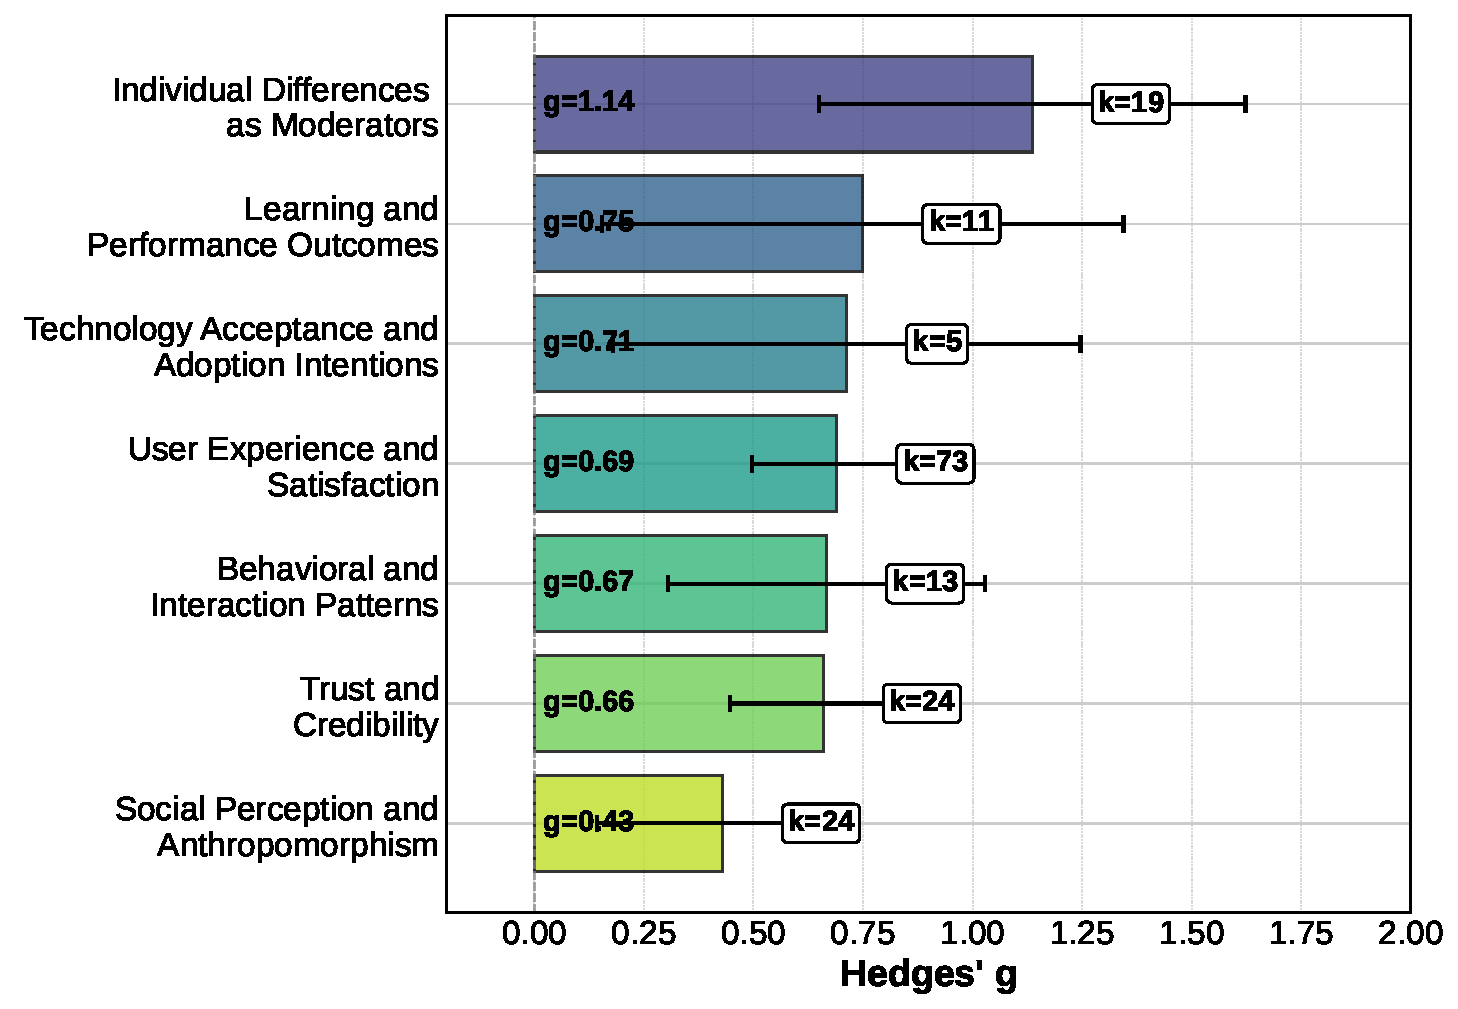
\includegraphics[width=0.6\linewidth]{Figures/figure3_outcome_categories.pdf}
    \caption{User outcomes for the anthropomorphic attributes.}
    \label{fig:outcomes}
\end{figure}

\subsection{Attribute-Outcome Specificity}

While behavioral attributes generally outperform demographic attributes, effect sizes vary substantially across outcomes. We analyzed which anthropomorphic attributes produce the strongest effects for which user outcomes (see Table \ref{tab:meta_matrix}). Estimates based on $k$ $<$ 5 are flagged as exploratory and excluded from design guidelines.

\subsubsection{Communication Style Improves UX}\label{sec:comm}

Communication style produced the largest effect on UX outcomes ($g$ = 1.73, 95\% CI [1.11, 2.35], $k$ = 13). These outcomes included satisfaction, usability, and enjoyment, while the examined attributes included politeness, formality, and natural conversational phrasing. The result indicates that how a CA communicates strongly shapes users' experience of receiving information through the interaction.

Communication style also produced a large effect on social perception ($g$ = 1.30, 95\% CI [0.58, 2.02], $k$ = 6). Communication strategies that made the interaction more natural and socially appropriate increased perceived humanness and social presence. Communication style therefore affects both how users experience information delivery and how they perceive the CA as its source.

\subsubsection{Visual Appearance Shows Outcome-Specific Patterns}

Visual appearance produced stronger effects on trust and credibility ($g$ = 0.63, 95\% CI [0.24, 1.02], $k$ = 5) than on UX outcomes ($g$ = 0.36, 95\% CI [$-$0.01, 0.73], $k$ = 12). Visual representations therefore appear to influence how users evaluate the CA as a credible information source more than how they assess the usability, satisfaction, or enjoyment of the interaction. This distinction indicates that visual design is most relevant when the goal is to strengthen confidence in the source of information, but is less effective as a standalone means of improving the overall user experience. 

\subsubsection{Demographic Identity and Learning Outcomes}

Demographic attributes, including assigned age, gender, ethnicity, and cultural identity, produced a moderate effect on UX outcomes ($g$ = 0.65, 95\% CI [0.24, 1.06], $k$ = 8). These attributes, therefore, influence how users experience the interaction, including their satisfaction, perceived usability, and enjoyment. However, their value depends on whether the assigned identity is relevant to the user and the interaction context. Demographic design should therefore support the intended relationship between the user, the CA, and the information it provides rather than serve as a default feature of general-purpose interfaces.

\subsubsection{Actions Work Across Contexts}

Action attributes, including proactivity, repair strategies, and interaction mechanisms, produced small-to-moderate effects on trust and credibility ($g$ = 0.30, 95\% CI [$-$0.10, 0.69], $k$ = 11) and behavioral and interaction outcomes ($g$ = 0.41, 95\% CI [$-$0.08, 0.90], $k$ = 7). These attributes influence how effectively the CA responds to users, manages misunderstandings, and sustains the exchange. Their effects, therefore, concern the process through which users receive and act on information, particularly whether the CA appears responsive and whether the interaction continues smoothly. Action attributes can support trust and engagement, but their effects are smaller and less certain than those observed for communication style.

\subsubsection{Personality Traits Show Dual Effectiveness}\label{sec:person}

Personality trait implementations produced moderate-to-large effects on UX ($g$ = 0.62, 95\% CI [0.29, 0.94], $k$ = 10). These effects concerned outcomes such as satisfaction, usability, and enjoyment. The pooled estimate indicates that personality traits can improve users' experience of interacting with and receiving information from a CA, although the variation in effects suggests that their influence depends on the specific implementation and context.

% Column types (put in preamble)
\newcolumntype{L}[1]{>{\raggedright\arraybackslash}p{#1}}
\newcolumntype{C}[1]{>{\centering\arraybackslash}p{#1}}

\begin{table*}[ht]
\centering
\caption{Meta-Analytic Effects of Anthropomorphic Attributes on User 
Outcomes. Hedges' \textit{g} values with significance markers 
(*** \textit{p} $<$ .001, ** \textit{p} $<$ .01, * \textit{p} $<$ .05). 
Cells marked $\dagger$ are based on $k$ $<$ 5 and are exploratory.}
\label{tab:meta_matrix}
\small
\setlength{\tabcolsep}{2.5pt}
\renewcommand{\arraystretch}{1.05}

\begin{tabular}{
L{0.245\textwidth}|
C{0.13\textwidth}
C{0.12\textwidth}
C{0.09\textwidth}
C{0.09\textwidth}
C{0.135\textwidth}
C{0.115\textwidth}
}
\hline
\textbf{Outcome} &
\multicolumn{3}{c}{\textbf{Behavioral}} &
\multicolumn{3}{c}{\textbf{Demographic}} \\
\cline{2-7}
&
{\small Comm. Styles} &
{\small Personality Traits} &
{\small Actions} &
{\small Identity} &
{\small Visual Representation} &
{\small Role \& Occupation} \\
\hline

UX and Satisfaction
 & {\cellcolor{green!20}1.73***} & {\cellcolor{yellow!20}0.62***} 
 & {\cellcolor{orange!20}0.35}
 & {\cellcolor{yellow!20}0.65**} & {\cellcolor{orange!20}0.36} & --- \\

Trust and Credibility
 & --- & --- & {\cellcolor{orange!20}0.30}
 & --- & {\cellcolor{yellow!20}0.63**} & --- \\

Learning and Performance Outcomes
 & --- & --- & {\cellcolor{green!20}0.87$\dagger$**}
 & {\cellcolor{green!20}0.98$\dagger$***} & --- & --- \\

Social Perception and Anthropomorphism
 & {\cellcolor{green!20}1.30***} & --- & {\cellcolor{red!20}0.08}
 & --- & --- & {\cellcolor{orange!20}0.28***} \\

Behavioral and Interaction Patterns
 & {\cellcolor{green!20}1.27$\dagger$} & --- & {\cellcolor{orange!20}0.41}
 & --- & --- & --- \\

Individual Differences as Moderators
 & --- & {\cellcolor{green!20}1.40} & {\cellcolor{red!20}0.19}
 & --- & {\cellcolor{green!20}3.14$\dagger$*} & --- \\
\hline
\end{tabular}
\end{table*}

\subsection{Triangulation from Multiple Syntheses} \label{sec:triang}

Three complementary synthesis methods validated the quantitative findings using the 373 non-calculable effects. Vote counting showed that 84.2\% of the directional effects were positive, exceeding chance expectations, $p$ $<$ .001 (binomial test). Fisher's combined probability test for 269 effects indicated that the pattern of statistical significance differs from chance, $\chi^2$(2$\times$269) = 1115.85, $p$ $<$ .001. Stouffer's Z-score method indicated predominantly positive effects, $Z$(269) = 8.84, $p$ $<$ .001. For effects without exact $p$-values, we assigned $p$ = 0.025 to findings reported as significant and $p$ = 0.50 to findings reported as non-significant. These substitutions allowed the tests to include studies that reported only significance thresholds. Sensitivity analyses using alternative substitutions (0.01--0.03 for significant effects and 0.40--0.60 for non-significant effects) produced the same result as both Fisher's test and Stouffer's method continued to indicate a statistically significant overall pattern of positive effects (all $p$ $<$ .001).

All three methods detected significant effects across all seven outcome categories (all $p$-values $<$ .01) and for both attribute types, with behavioral attributes consistently showing stronger evidence. The agreement across methods indicates that the overall result does not depend on one form of analysis.

The analysis of implementation patterns across the 79-article corpus revealed that research practice aligns with the findings on effectiveness. Behavioral attributes dominate design choices: communication style appeared in 50.0\% of studies and personality traits in 48.3\%, compared to demographic attributes (37.9\%), assigned roles (24.1\%), and visual appearance (15.5\%). Overall, behavioral attributes appeared significantly more frequently than demographic attributes (77.6\% versus 41.4\%), $z$ = 3.97, $p$ $<$ .001, Cohen's $h$ = 0.76.

Publication-bias analysis produced a lower adjusted overall effect ($g$ = 0.48, 95\% CI [0.33, 0.63]) than the primary three-level estimate ($g$ = 0.68, 95\% CI [0.38, 0.98]). Both estimates indicate that anthropomorphic design has a positive overall effect on user outcomes, although the adjusted result suggests a more moderate magnitude.

Across the 542 analyzed effects, the main finding is that the effectiveness of anthropomorphic design depends more on the attribute and intended outcome than on anthropomorphism alone. Communication style ($g$ = 1.15, $k$ = 25) and personality traits ($g$ = 1.07, $k$ = 19) produced the largest attribute-level effects. UX ($g$ = 0.69, $k$ = 73), trust and credibility ($g$ = 0.65, $k$ = 24), and learning and performance ($g$ = 0.75, $k$ = 11) showed the strongest outcome-level effects, while social perception showed a smaller effect ($g$ = 0.43, $k$ = 24). These results indicate that designers should prioritize how the CA communicates and behaves and select representational attributes based on the specific information and interaction outcomes they intend to improve.

\section{Discussion}

\subsection{Theoretical Implications}

This study contributes to CA anthropomorphism research by identifying which specific attributes matter most, for which outcomes, and to what degree. Our findings are consistent with the CASA framework \parencite{nass1994computers}, which predicts that social cues in computer interfaces trigger automatic social responses in users. Both behavioral and representational anthropomorphic attributes produced positive effects in all synthesis methods. This pattern aligns with CASA's core claim that minimal human-like cues are sufficient to elicit social responses, a claim that appears to hold even for LLM-based CAs, where the conversational quality of those cues is substantially higher than in legacy systems.

An important qualification applies. \textcite{koger2023casa} found that users no longer responded socially to desktop computers after extended exposure, raising the possibility that CASA effects are historically contingent and strongest for emerging technologies. The studies in this corpus predominantly examine LLM-based CAs at a period when users are still forming interaction scripts with these systems. Whether the effects documented here persist as LLM-based CAs become normalized remains an open empirical question. Our findings are consistent with CASA predictions but do not test the mechanisms underlying them or their durability.

Within these categories, heterogeneity in effectiveness is substantial. Communication style showed the strongest effects among behavioral attributes, while visual appearance produced larger effects than demographic identity assignments among representational attributes. These differences indicate that implementation choices within anthropomorphic design influence outcomes as much as the broad behavioral-versus-representational distinction. The high within-study heterogeneity, which exceeds between-study heterogeneity in the three-level decomposition, confirms that the same study can produce very different effects depending on which attribute-outcome combination is examined. Possible explanations for this variability include implementation quality, interaction duration, task context, and user characteristics, none of which were analyzable as moderators in the current dataset.

This study's primary theoretical contribution is to quantify these effects and identify which specific anthropomorphic attributes result in the strongest outcomes. Communication style and coherent personality expression emerge as particularly productive design targets. These results support placing greater emphasis on how the agent continuously acts rather than on what the agent appears to be, though the data do not entirely support dismissing representational design. Representational attributes produced moderate-to-large effects in their own right, and the behavioral-representational magnitude difference did not reach significance in formal moderation testing.

Prior meta-analyses on anthropomorphism in CAs has established that human-like social cues produce positive effects on user outcomes \parencite{klein_effects_2025,chaves2021should}. The present study extends this line of work by distinguishing behavioral from representational attributes, mapping effects to specific outcome categories, and applying a multilevel model that accounts for the nested structure of effects within studies. These methodological additions provide more precise guidance on which attributes to prioritize for which design goals, moving beyond the aggregate estimates reported in prior syntheses.

Beyond identifying which attributes matter, this study provides tentative benchmark effect sizes for anthropomorphic CA design research. Individual effect sizes in the corpus ranged from small negative to very large positive values ($M$ = 0.79, $Mdn$ = 0.53, $SD$ = 1.20, range = $-$1.39 to 7.09). These descriptives characterize the realistic distribution of effects produced by empirical studies in this area, including the long right tail driven by communication style and personality implementations. Researchers designing anthropomorphic CA studies can use these values as tentative benchmarks for power analysis and effect size expectations, treating the median as the conservative planning estimate and the mean as the optimistic upper bound. The field has lacked this kind of distributional reference point, and its absence has made it difficult to evaluate whether new empirical findings fall within, above, or below the range observed in prior work.

\subsection{Practical Implications}

Based on our findings, we propose five design guidelines (DGs) for anthropomorphism in CAs. Each guideline identifies the sub-theme and the quality of the evidence. Guidelines are grounded solely in reliable estimates. Estimates based on fewer than five effects are noted as exploratory and excluded from prescriptive recommendations.

\textbf{DG1: Prioritize communication style} (Section \ref{sec:beh}). Communication style is the single most effective anthropomorphic attribute in the corpus, producing large effects on both UX and social perception. Designers should invest in natural language generation, formality adaptation, and politeness calibration. CAs that employ contextually appropriate language and an adaptive tone produce substantially better outcomes than those that rely on uniform or scripted communication. This guideline rests on a reliable estimate based on twenty-five effects.

\textbf{DG2: Implement coherent personality} (Section \ref{sec:person}). Personality traits significantly affect user outcomes, particularly in UX. Coherent personality expression, meaning consistent behavioral patterns in every response, matters more than the specific traits chosen. An agreeable CA should prioritize cooperative phrasing throughout. An extroverted CA should consistently initiate and sustain engagement. Inconsistent personality expression breaks the social contract and is likely the reason that a significant proportion of effects in this category did not reach significance. This guideline rests on a reliable estimate based on nineteen effects.

\textbf{DG3: Build proactive responsiveness} (Section \ref{sec:beh}). Behavioral pattern attributes, including proactive dialogue actions, intelligent turn-taking, and repair strategies, yield consistent, moderate effects across diverse outcome categories. Every effect examined for trust and behavioral patterns outcomes reached significance, indicating reliable returns despite moderate magnitudes. Designers should implement CAs that anticipate user needs without seeming intrusive and respond appropriately when misunderstandings occur. This guideline rests on a reliable estimate based on forty-five effects.

\textbf{DG4: Match anthropomorphic attributes with intended outcomes} (Section \ref{sec:out}). Attribute selection should follow the intended outcome. Communication style has the most reliable effects on UX and social perception, making it the priority for service and companionship interfaces. Visual appearance influences trust and credibility more than UX, making it more valuable in contexts where perceived trustworthiness matters. Demographic identity produces moderate effects on UX and should be applied when user-agent demographic alignment is contextually relevant. 
% Exploratory estimates, including those for demographic identity on learning outcomes and visual appearance as a moderator, are not included in this guidance.

\textbf{DG5: Manage expectations for behavioral and adoption outcomes} (Section \ref{sec:out}). Anthropomorphism produces its strongest effects on perceptual outcomes such as UX and social presence. Effects on adoption intentions and observable behavioral patterns are more modest. A CA that communicates warmly but fails at core tasks will not overcome adoption barriers through persona alone. Designers are encouraged to treat anthropomorphic design as a complement to functional quality and to communicate realistic expectations about its contribution to adoption metrics.

\subsection{Limitations and Future Directions}

Several limitations constrain the interpretation and generalizability of these findings.

First, the corpus is predominantly text-centric. The search strategy retrieved fewer studies on voice and embodied agents than the broader literature contains, and the design guidelines derived here should not be extended to those modalities without further empirical evidence. Behavioral attributes such as prosody, gaze, and gesture, which are central to embodied and voice CA design, are absent from most studies in this corpus \parencite{cassell2000embodied,bickmore2005relational}.

Second, publication bias affects the estimated magnitude of the results. Egger's test indicated significant funnel-plot asymmetry (intercept = 1.72, $SE$ = 0.04, $t$(167) = 40.23, $p$ $<$ .001), suggesting that the corpus over-represents larger positive effects. Duval and Tweedie's trim-and-fill procedure estimated 23 missing studies and produced an adjusted pooled effect of $g$ = 0.48 (95\% CI [0.33, 0.63]), which was 34\% lower than the unadjusted two-level estimate. The one-effect-per-study sensitivity analysis also produced a lower estimate ($g$ = 0.64, 95\% CI [0.36, 0.91]) than the full two-level model. These analyses indicate that selective reporting and small-study effects may have increased the observed magnitudes. However, the three-level model, the adjusted estimate, the one-effect-per-study analysis, and the syntheses of non-calculable effects all indicate a positive overall relationship between anthropomorphic design and user outcomes. The direction of the finding is therefore consistent across analyses, although the unadjusted effect sizes should not be treated as expected effects for individual implementations.

Third, heterogeneity is considerable. The wide prediction interval indicates that the effect in a new study may range from negative to strongly positive. The three-level model shows that much of this variation occurs within studies, meaning that the effects differ according to the particular attribute and outcome examined. The pooled estimate, therefore, describes the average relationship across the literature but does not replace attribute-specific and outcome-specific estimates. Future studies should report implementation details more consistently so that meta-analyses can examine whether interaction duration, task context, user group, and implementation quality explain this variation.

Fourth, the corpus spans both pre-LLM and LLM-based studies. Whether effect sizes differ systematically between these periods cannot be examined cleanly because studies often do not specify whether the underlying CA uses a large language model. Future meta-analyses should code LLM use as a categorical moderator, given that LLM-based CAs may produce different anthropomorphic effects through greater language fluency and contextual adaptation than rule-based predecessors \parencite{amin2024chatgpt}.

Fifth, the interaction between behavioral and representational attributes remains unexamined. The current data cannot determine, for example, whether the effect of communication style increases when it is paired with a coherent demographic identity or visual representation. Future studies should test these combinations directly, and subsequent meta-analyses should examine whether particular combinations produce additive, reinforcing, or conflicting effects.

Future research should also examine how implementation quality, interaction duration, task characteristics, user characteristics, and cultural context affect the relationship between anthropomorphic design and user outcomes. Longitudinal designs are particularly needed because most studies in the corpus examined single-session interactions, leaving the durability of these effects under repeated use unclear. We make our coding sheet available for researchers to extend as further evidence becomes available\footnote{\href{https://osf.io/7rj6f/overview?view_only=35b327583fee4222b5b336465107580c}{https://bit.ly/4nn1NhZ}}.

\subsection{Ethical Considerations of Anthropomorphic Design in CAs}

The anthropomorphic design of CAs raises ethical concerns that practitioners must address before deployment.

The most direct risk is para-social dependency. Human-like communication can produce emotional attachments to agents incapable of genuine reciprocation \parencite{chaves2021should}. %This risk is not hypothetical. 
Documented cases of users forming deep emotional dependencies on anthropomorphic CAs have resulted in real psychological harm \parencite{laura_kuenssberg_mothers_2025}. The communication style and personality effects documented in this study, while beneficial for UX and social perception, are precisely the attributes that drive para-social attachment. The most effective CAs, according to the metrics in this study, are also the ones that carry the highest dependency risk.

A second risk is manipulation. Anthropomorphism lowers users' critical evaluation of CA outputs and increases compliance with suggestions that users would otherwise scrutinize \parencite{chaves2021should}. This serves as an inadvertent mechanism for manipulation. Users who perceive a CA as a social entity are more likely to trust its outputs and less likely to detect errors or biases. The substantial effect of communication style on social perception documented here means that well-designed language can produce strong impressions of competence and warmth that may exceed the system's actual capabilities.

A third risk concerns demographic representation. Assigning demographic attributes to CAs, particularly gender and ethnicity, risks encoding and reinforcing social stereotypes. Pairing female presentation with service roles, or associating demographic attributes with authority markers, can reproduce patterns of bias at scale, given the reach of deployed CA systems. The finding that demographic attributes produce meaningful effects on user outcomes also means that these design choices are not neutral.

Designers should treat the disclosure of artificial identity and the consistency between stated and actual capabilities as ethical obligations across all deployment contexts. The design guidelines in this study are recommendations for effectiveness. Practitioners are urged to weigh them against the dependency, manipulation, and representation 
risks described here before making deployment decisions.


\section{Conclusion}

This meta-analysis shows that anthropomorphic design generally improves user outcomes, but the effect depends on the attribute used and the targeted outcome. Communication style and personality traits produced the largest effects, indicating that how a CA communicates and behaves matters more than simply giving it a human-like appearance or identity. Visual appearance was more relevant to trust and credibility than to UX, while demographic identity mainly affected users' experience of the interaction. Anthropomorphic design, therefore, influences both how users receive information and how they evaluate the CA as its source. Designers should prioritize adaptive communication and coherent personality expression, while selecting visual and demographic attributes only when they support a specific interaction or information goal. These conclusions apply primarily to text-based CAs; further research is needed to determine whether the same relationships hold for voice-based and embodied agents.

\printbibliography[title={References}]
\end{document}

